\begin{figure}[t]\centering
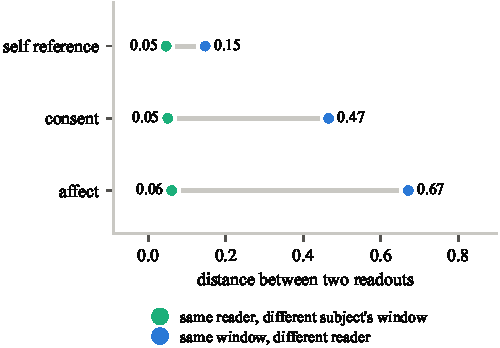
\includegraphics[width=\columnwidth]{figures/crossing}
\caption{A readout tracks the reader more closely than it tracks the window.
Each bar spans two distances measured on the same probe: how far apart two
readouts sit when the window changes and the reader does not, against how far
apart they sit when the reader changes and the window does not. The second is
an order of magnitude larger on every probe. Table~\ref{tab:crossing} adds the
comparison that rules out privileged access.}
\label{fig:crossing}
\end{figure}
